Die Analysis ist ein wichtiges Teilgebiet der Mathematik, dessen Inhalte sich nicht genau abgrenzen lassen. Grob gesagt befasst sie sich mit der Untersuchung von Eigenschaften von Funktionen. Viele Methoden der Analysis haben wichtige Anwendungen in Naturwissenschaft und Technik.

Eine zentrale Grundlage bildet dabei der Grenzwertbegriff.

Im Folgenden beschäftigen wir uns daher zunächst mit Grenzwerten von Funktionen.

\section{Grenzwerte von Funktionen}
\subsection{Grenzwerte für $x \to \pm \infty$}
\paragraph{Einführungsaufgabe}
\begin{enumerate}
    \item Benutzen Sie Geogebra, um den Graphen der Funktion $f(x) = \frac{3x^2+x-2}{2x^2-5x+9}$ zu zeichnen.
    \item 	Was vermuten Sie: Was passiert mit den Werten von $f$, wenn $x$ immer grösser wird?
    \item Zeigen Sie Ihre Vermutung mit Hilfe einer geschickten Termumformung.
    \item Was passiert, wenn x immer kleiner wird, also für $x\rightarrow-\infty$?
    \item Bestimmen Sie die beiden Grenzwerte $\lim_{x\to \infty}g(x)$ und $\lim_{x\to -\infty}g(x)$ der Funktion
          \[g(x) =\dfrac{2^x}{2^x+1}\]
\end{enumerate}
\clearpage
Die Werte der Funktion $f(x) = \frac{3x^2+x-2}{2x^2-5x+9}$ scheinen auf den ersten Blick für $x \to \infty$ gegen die Zahl $1.5$ zu gehen. Gewissheit erlangt man aber erst durch eine Termumformung:

\begin{align*}
    f(x) = \frac{3x^2+x-2}{2x^2-5x+9} = \frac{x^2\left(3+\frac{1}{x}-\frac{2}{x^2}\right)}{x^2\left(2-\frac{5}{x}+\frac{9}{x^2}\right)}=\frac{3+\frac{1}{x}-\frac{2}{x^2}}{2-\frac{5}{x}+\frac{9}{x^2}}
\end{align*}
Für sehr grosse Werte von $x$ nähern sich die Terme $\frac{1}{x}$, $\frac{2}{x^2}$, $\frac{5}{x}$ und $\frac{9}{x^2}$ der Zahl $0$. Für $x\to \infty$ erhält man somit:
\[
    \lim_{x\to \infty}f(x)=\frac{3+0-0}{2-0+0}=\frac{3}{2}
\]
Die Technik im Beispiel ist eine Anwendung der sogenannten Grenzwertsätzen:
\begin{theo}[Grenzwertsätze]{}{}
    Besitzen die Funktionen $f\left(x\right)$ und $g\left(x\right)$ Grenzwerte für $x\rightarrow+\infty$ so sind auch die Funktionen $f\left(x\right)\pm g\left(x\right),$ $f\left(x\right)\cdot g\left(x\right)$ und, sofern $\displaystyle\lim_{x\to \infty}g\left(x\right)\neq0$, auch die Funktion $\frac{f\left(x\right)}{g\left(x\right)}$ konvergent.
    Für die Grenzwerte gilt

    \begin{align*}
        \lim_{x \to \infty} (f(x) \pm  g(x))               & = \lim_{x\to\infty} f(x) \pm \lim_{x\to\infty} g(x)      \\
        \lim_{x \to \infty} (f(x) \cdot  g(x))             & = \lim_{x\to\infty} f(x) \cdot \lim_{x\to\infty} g(x)    \\
        \lim_{x \to \infty} \left(\frac{f(x)}{g(x)}\right) & = \frac{\lim_{x\to\infty} f(x)}{ \lim_{x\to\infty} g(x)} \\
    \end{align*}
    Der Satz gilt auch für den Fall $x \to -\infty$
\end{theo}
Beweis: Siehe entsprechneder Beweis im Kapitel \glqq Grenzwerte von Folgen und Reihen\grqq{}

\subsubsection{Übungen}
\begin{enumerate}
    \item Bestimmen Sie, sofern vorhanden, den Grenzwert des Funktionsterms für $x \to \infty$.
          \begin{enumerate}
              \item $\lim\limits_{x \to \infty} \frac{x}{3x - 1}$
              \item $\lim\limits_{x \to \infty} \frac{1 - x^2}{x}$
              \item $\lim\limits_{x \to \infty} \frac{3x^7 - 4x^5}{2x^7 + 7x^6}$
              \item $\lim\limits_{x \to \infty} \frac{3 - x^3}{2x^3 + x^2}$
          \end{enumerate}
    \item Welchen Wert hat $\lim\limits_{x \to \infty} f(x)$ und $\lim\limits_{x \to -\infty} f(x)$?

          \begin{enumerate}
              \item $f(x) = \frac{2 + 3 \cdot 2^x}{2^x \cdot 4 - 1}$
              \item $f(x) = \frac{5^{-x} + 3}{8 - 2 \cdot 5^{-x}}$
          \end{enumerate}

    \item
          Berechne

          \begin{enumerate}
              \item $\lim\limits_{x \to \infty} \frac{x^3 + \sin(x)}{x^3}$
              \item $\lim\limits_{x \to -\infty} \frac{x^2 - \sin(x)}{x^3}$
              \item $\lim\limits_{x \to \infty} \frac{\cos(x) - 3x}{1 - 2x}$
          \end{enumerate}
    \item Bestimmen Sie die beiden Grenzwerte und vergleiche.

          \begin{enumerate}
              \item $\lim\limits_{x \to \infty} \frac{2x^6 - 3x^5 + 7x^3 + 4x - 8}{5x^6 + 8x^5 - 9x^4 + 11x^2}$, \quad $\lim\limits_{x \to -\infty} \frac{2x^6 - 3x^5 + 7x^3 + 4x - 8}{5x^6 + 8x^5 - 9x^4 + 11x^2}$
              \item $\lim\limits_{x \to \infty} \frac{10x^8 - 4x^7 + 12}{x^9 + 3x^6 + 4}$, \quad $\lim\limits_{x \to -\infty} \frac{10x^8 - 4x^7 + 12}{x^9 + 3x^6 + 4}$
              \item  $\lim\limits_{x \to \infty} \frac{10x^8 - 4x^7 + 12}{x^7 + 3x^6 + 4}$, \quad $\lim\limits_{x \to -\infty} \frac{10x^8 - 4x^7 + 12}{x^7+ 3x^6 + 4}$
              \item   $\lim\limits_{x \to \infty} \frac{10x^8 - 4x^7 + 12}{ 3x^6 + 4}$, \quad $\lim\limits_{x \to -\infty} \frac{10x^8 - 4x^7 + 12}{3x^6 + 4}$
              \item $\lim\limits_{x \to \infty} \frac{\sqrt{x + 1}}{x - 1}$, \quad $\lim\limits_{x \to -\infty} \frac{\sqrt{x + 1}}{x - 1}$
              \item $\lim\limits_{x \to \infty} \frac{x^9 + x^4}{e^x}$, \quad $\lim\limits_{x \to -\infty} \frac{x^9 + x^4}{e^x}$
          \end{enumerate}
    \item Bestimmen Sie die Parameter $a, b$ und $c$ so, dass gilt:
          \[ \lim\limits_{x \to \infty} \frac{ax^b + 4x^5 + cx^3 - 1}{2x^3 - 11x^2 + 5} = 3. \]
    \item  Gegeben ist der Funktionsterm $f(x) = \frac{4x^4 - 6x^3 + 7}{2x^m + 5x + 1}$. Bestimmen Sie den Exponenten $m \in \mathbb{N}_0$ so, dass die folgenden Grenzwerte resultieren, oder erklären Sie, weshalb es kein $m$ mit diesem Grenzwert gibt.
          \begin{enumerate}
              \item $\lim\limits_{x \to \infty} f(x) = 2$
              \item $\lim\limits_{x \to \infty} f(x) = 0$
              \item $\lim\limits_{x \to -\infty} f(x) = -2$
              \item $\lim\limits_{x \to -\infty} f(x) = -\infty$
              \item $\lim\limits_{x \to -\infty} f(x) = \infty$
          \end{enumerate}
\end{enumerate}

\clearpage
\subsubsection*{Lösungen}
\begin{enumerate}
    \item

          \begin{enumerate}
              \item $\lim\limits_{x \to \infty} \frac{x}{3x - 1} = \frac{1}{3}$
              \item $\lim\limits_{x \to \infty} \frac{1 - x^2}{x} = -\infty$
              \item $\lim\limits_{x \to \infty} \frac{3x^7 - 4x^5}{2x^7 + 7x^6} = \frac{3}{2}$
              \item $\lim\limits_{x \to \infty} \frac{3 - x^3}{2x^3 + x^2} = -\frac{1}{2}$
          \end{enumerate}

    \item

          \begin{enumerate}
              \item $f(x) = \frac{2 + 3 \cdot 2^x}{2^x \cdot 4 - 1}$, Grenzwert für $x\to \infty$: $\frac{3}{4}$, Grenzwert für $x\to-\infty$: $-2$
              \item $f(x) = \frac{5^{-x} + 3}{8 - 2 \cdot 5^{-x}}$, Grenzwert für $x\to \infty$: $\frac{3}{8}$, Grenzwert für $x\to-\infty$: $-\frac{1}{2}$
          \end{enumerate}

    \item

          \begin{enumerate}
              \item $\lim\limits_{x \to \infty} \frac{x^3 + \sin(x)}{x^3} = 1$
              \item $\lim\limits_{x \to -\infty} \frac{x^2 - \sin(x)}{x^3} = 0$
              \item $\lim\limits_{x \to \infty} \frac{\cos(x) - 3x}{1 - 2x} = \frac{3}{2}$
          \end{enumerate}

    \item

          \begin{enumerate}
              \item $\lim\limits_{x \to \infty} \frac{2x^6 - 3x^5 + 7x^3 + 4x - 8}{5x^6 + 8x^5 - 9x^4 + 11x^2} = \frac{2}{5}$, $\lim\limits_{x \to -\infty} \frac{2x^6 - 3x^5 + 7x^3 + 4x - 8}{5x^6 + 8x^5 - 9x^4 + 11x^2} = \frac{2}{5}$
              \item $\lim\limits_{x \to \infty} \frac{10x^8 - 4x^7 + 12}{x^9 + 3x^6 + 4} = 0$, $\lim\limits_{x \to -\infty} \frac{10x^8 - 4x^7 + 12}{x^9 + 3x^6 + 4} = 0$
              \item   $\lim\limits_{x \to \infty} \frac{10x^8 - 4x^7 + 12}{x^7 + 3x^6 + 4} = \infty$, \quad $\lim\limits_{x \to -\infty} \frac{10x^8 - 4x^7 + 12}{x^7+ 3x^6 + 4}=- \infty$
              \item   $\lim\limits_{x \to \infty} \frac{10x^8 - 4x^7 + 12}{ 3x^6 + 4}= \infty$, \quad $\lim\limits_{x \to -\infty} \frac{10x^8 - 4x^7 + 12}{3x^6 + 4}= \infty$
              \item $\lim\limits_{x \to \infty} \frac{\sqrt{x + 1}}{x - 1} = 0$, $\lim\limits_{x \to -\infty} \frac{\sqrt{x + 1}}{x - 1}$ gibt es nicht
              \item $\lim\limits_{x \to \infty} \frac{x^9 + x^4}{e^x} = 0$, $\lim\limits_{x \to -\infty} \frac{x^9 + x^4}{e^x} = -\infty$
          \end{enumerate}

    \item $a = -4$, $b = 5$, $c = 6$.

    \item    \begin{enumerate}
              \item $\lim\limits_{x \to \infty} f(x) = 2$, Lösung: $m = 4$
              \item $\lim\limits_{x \to \infty} f(x) = 0$, Lösung:  $m>4$
              \item $\lim\limits_{x \to -\infty} f(x) = -2$, Lösung: nicht möglich
              \item $\lim\limits_{x \to -\infty} f(x) = -\infty$, Lösung: $m\in \{0, 1, 3\}$
              \item $\lim\limits_{x \to -\infty} f(x) = \infty$, Lösung: $m =2$
          \end{enumerate}

\end{enumerate}

\clearpage
\subsection{Grenzwerte einer Funktion an einer Stelle $a\in \mathbb{R}$}
\subsubsection*{Einführungsaufgabe}
Untersuchen Sie die Funktion $f(x)=\frac{x^3+10x^2-24x}{7x-14}$.
\begin{enumerate}
    \item Wieso ist die Funktion an der Stelle $x=2$ nicht definiert?
    \item Zeichnen Sie die Funktion mit \href{https://www.geogebra.org/calculator}{Geogebra}
    \item Definieren Sie in Geogebra einen `Laufpunkt' auf dem Graphen von $f$, indem Sie P=(a, f(a)) tippen. Geogebra erstellt automatisch einen Schieberegler, mit dem Sie die $x$-Koordinate von $P$ verändern können.
    \item  Beobachten Sie, was mit $P$ passiert, wenn $a$ sich der Zahl 2 nähert.
    \item  Was vermuten Sie ist der Wert des Grenzwertes $\lim\limits_{x\to 2} f(x)$?
    \item  Wie kann man diesen Grenzwert anhand der Funktionsgleichung berechnen?
          %\item  Wenn man etwas rauszoomt, sieht man, dass der Graph von $f$ eine bekannte Form hat. Können Sie das anhand der Funktionsgleichung erklären?
\end{enumerate}
\clearpage
Mit der Einführungsaufgabe haben wir ein Beispiel dafür, wie man sich den Grenzwert einer Funktion für x gegen eine Zahl vorstellen muss. Auch für diesen Grenzwertbegriff gibt es eine präzise, mathematische Definition, wir verzichten aber hier vorerst darauf und beschränken uns auf eine etwas ungenauere, dafür verständlichere Variante:

\begin{deff}[Grenzwert einer Funktion $x \to a$]{}{}
    Eine Zahl $g$ heisst Grenzwert der Funktion $f$ für $x$ gegen $a$, falls alle Funktionswerte $f\left( x\right)$ beliebig wenig von $g$ abweichen, sobald $x$ entsprechend nahe bei $a$ liegt, aber verschieden von $a$ ist. Notation:
    \begin{equation*}
        \lim_{x \to a} f(x) = g
    \end{equation*}
\end{deff}
Mittels GeoGebra konnten wir bereits eine Vermutung für den Grenzwert $\lim\limits_{x\to 2} f(x)$ formulieren.

Wie lässt sich diese Vermutung jedoch absichern? GeoGebra berechnet lediglich Funktionswerte für $x$ in der Nähe von $2$. Es gibt jedoch Zahlen, die noch wesentlich näher bei $2$ liegen als die betrachteten.

Wieder hilf eine Termumformung:
\begin{align*}
    \frac{x^3+10x^2-24x}{7x-14} = \frac{x(x^2+10x-24)}{7(x-2)} = \frac{x(x-2)(x+12)}{7(x-2)}\stackrel{x\neq 2}{=}\frac{x(x+12)}{7}
\end{align*}

Die beiden Terme ganz links und ganz rechts liefern für alle Werte von $x$ das gleiche Resultat mit einer Ausnahme: Für $x=2$ ist der Term links nicht definiert, der rechts aber schon. Bildlich gesprochen stimmen die Graphen der beiden Funktionen $f(x)=\frac{x^3+10x^2-24x}{7x-14}$ und $g(x)=\frac{x(x+12)}{7}$ überall überein – nur das der Graph von $f$ an der Stelle $x=2$ ein Loch aufweist, während jener von $g$ durchgängig ist.
Damit gilt
$$\lim_{x\rightarrow2} \frac{x^3+10x^2-24x}{7x-14} = \lim_{x\rightarrow2} \frac{x(x+12)}{7} =\frac{2\cdot (2+12)}{7} = 4$$

\subsubsection{Übungen}
Bestimmen Sie den Grenzwert.
\begin{multicols}{3}
    \begin{enumerate}
        \item $\lim\limits_{x \to 1} \frac{x^2 + 4x - 5}{x^2 - 1}$
        \item $\lim\limits_{x \to 1} \frac{x^2 + 4x - 5}{x^2 - 2x + 1}$
        \item $\lim\limits_{x \to -9} \frac{x^2 + 7x - 18}{x^2 - 81}$
        \item $\lim\limits_{x \to -4} \frac{x + 6}{x^2 - 4}$
        \item $\lim\limits_{x \to -2} \frac{12x^2 + 24x}{x^2 + 10x + 16}$
        \item $\lim\limits_{x \to 2} \frac{3x^2 - 6x}{6 - 5x + x^2}$
        \item $\lim\limits_{x \to 4} \frac{2x^2 - 14x + 24}{12x - 7x^2 + x^3}$
    \end{enumerate}
\end{multicols}
\clearpage

\subsubsection*{Lösungen}
\begin{multicols}{2}
    \begin{enumerate}
        \item $3$
        \item divergent ($\pm\infty$)
        \item $\dfrac{11}{18}$
        \item $\dfrac{1}{6}$
        \item $-4$
        \item $-6$
        \item $\dfrac{1}{2}$
    \end{enumerate}
\end{multicols}
\clearpage

\subsection{Linksseitige und rechtsseitige Grenzwerte, Stetigkeit}
\subsubsection*{Einführungsaufgabe}
Wir untersuchen die Funktion:
$$f(x) = x\cdot \sqrt{1+\frac{1}{x^2}}$$

\begin{enumerate}
    \item An welcher Stelle ist die Funktion nicht definiert?
    \item Was passiert, wenn $x$ sich der Definitionslücke nähert?
    \item Zeichnen Sie den Graphen von $f$ mit Geogebra und fügen Sie ihn hier unten an (Wurzeln können mit dem Befehl \glqq sqrt\grqq{} oder mit \glqq hoch 0.5\grqq{} eingegeben werden).
\end{enumerate}
\clearpage
Für die Funktion aus der Einführungsaufgabe gilt: Je nachdem ob $x$ von links oder rechts gegen $0$ strebt, strebt der Funktionswert gegen $-1$ oder gegen $1$.
\begin{figure}[H]
    \centering
    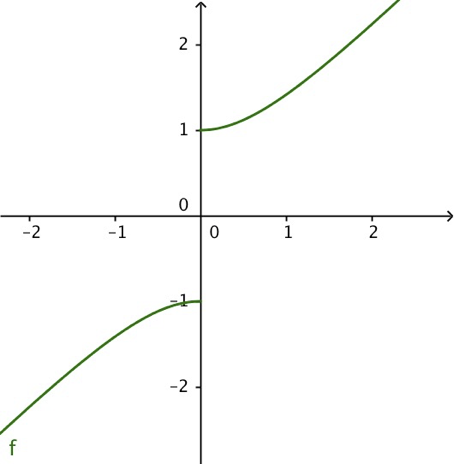
\includegraphics[scale=0.3]{im/Links_rechtsseitigerGrenzwert.png}
\end{figure}
Man spricht in diesem Fall vom links- bzw rechtsseitigem Grenzwert und schreibt
$$\lim_{x\uparrow 0} f(x) = -1 \quad \mathrm{oder}  \lim_{x\rightarrow 0^-} f(x) = -1 $$
beziehungsweise
$$\lim_{x\downarrow 0} f(x) = 1 \quad \mathrm{oder}  \lim_{x\rightarrow 0^+} f(x) = 1 $$

\begin{example}
    Wie bestimmt man den links- und den rechtsseitigen Grenzwert der Funktion $f(x) = x\cdot \sqrt{1+\frac{1}{x^2}}$ für $x\to 0$ ohne GeoGebra zu verwenden?

    
\end{example}

Der folgende Satz erklärt den Zusammenhang zwischen links- und rechtsseitigem Grenzwert und dem Grenzwert $x\rightarrow a$:

\begin{theo}{}{}
    Wenn der links- und der rechtsseitige Grenzwert übereinstimmen, dann existiert auch DER Grenzwert und es gilt
    \begin{align*}
        \lim_{x\rightarrow a}{f\left(x\right)}=\lim_{x\uparrow a}{f\left(x\right)}=\lim_{x\downarrow a}{f\left(x\right)}.
    \end{align*}
    Wenn der links- und der rechtsseitige Grenzwert nicht übereinstimmen, dann existiert der Grenzwert $\lim_{x\rightarrow a}{f\left(x\right)}$ nicht.
    \begin{align*}
        \lim_{x\uparrow a}{f\left(x\right)}\neq\lim_{x\downarrow a}{f\left(x\right)}\ \ \Longrightarrow\ \ \lim_{x\rightarrow a}{f\left(x\right)}\ \mathrm{existiert\ nicht}.
    \end{align*}
\end{theo}
\begin{example}
    Die \textit{Aufrundungsfunktion} $g\left(x\right)=\left\lceil x\right\rceil$ rundet jede Zahl auf die kleinste ganze Zahl grösser oder gleich $x$ auf.

    $\lim_{x\uparrow 42} \lceil x\rceil = ? , \quad \lim_{x\downarrow 42} \lceil x\rceil = ? $, Graph?
    \kariert{45}
\end{example}
\clearpage

\subsubsection{Stetigkeit}
Mit der Aufrundungsfunktion und der Funktion in der Einführungsaufgabe haben Sie Funktionen kennengelernt, die an gewissen Stellen Sprünge machen. Die meisten Funktionen, die Sie bisher angetroffen haben, hatten keine solche Sprungstellen. Wenn eine Funktion keine Sprungstelle hat, nennt man sie stetig. Genauer:
\begin{deff}[Stetigkeit]{}{}
    Eine Funktion $f$ mit Definitionsbereich $\mathbb{D}$ heisst \textbf{stetig an der Stelle $a \in \mathbb{D}$}, wenn
    \begin{align*}
        \lim_{x\uparrow a}{f\left(x\right)}=\lim_{x\downarrow a}{f\left(x\right)}=f\left(a\right)
    \end{align*}
    Eine Funktion $f$ heisst stetig, wenn sie an \textit{jeder} Stelle $a \in \mathbb{D}$ stetig ist.
\end{deff}
\begin{example}
    \begin{minipage}{0.6\textwidth}
        Die Quadratfunktion $f(x)=x^2$ ist stetig. Der Graph weist keinerlei Sprünge auf.
    \end{minipage}
    \begin{minipage}{0.3 \textwidth}
        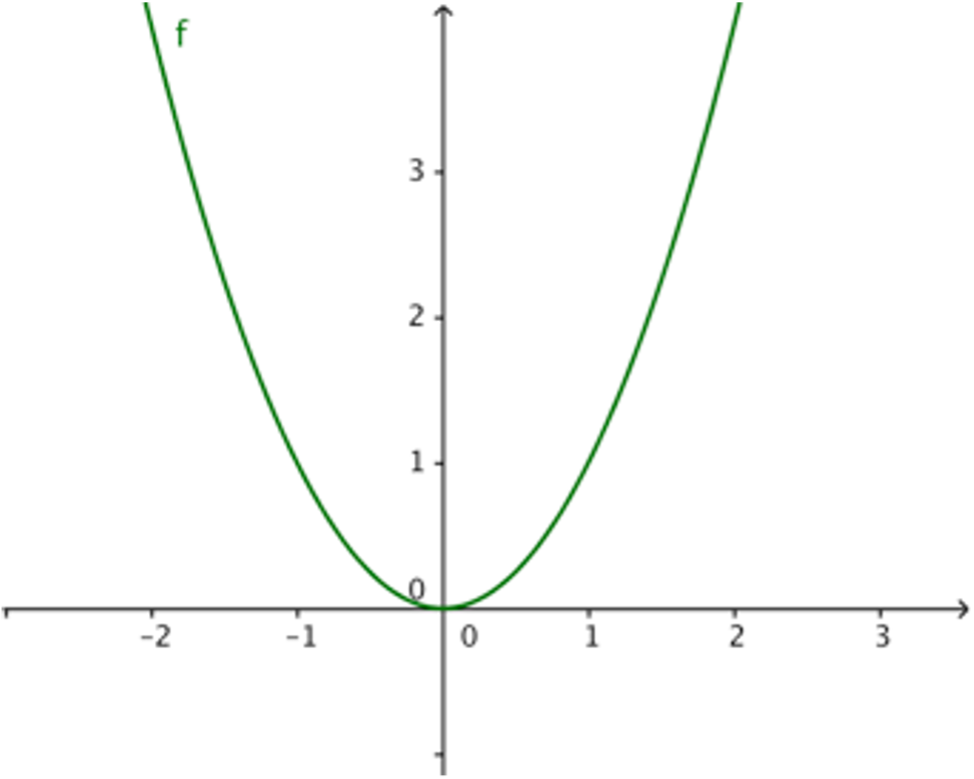
\includegraphics[scale =0.5]{im/QuadrFktStetig.png}
    \end{minipage}
\end{example}

\begin{example}
    \begin{minipage}{0.6\textwidth}
        Die Vorzeichen-Funktion
        \begin{align*}
            \mathrm{sgn}(x) = \begin{cases}
                                  1,  & \text{falls } x> 0 \\
                                  0,  & \text{falls } x= 0 \\
                                  -1, & \text{falls } x< 0 \\
                              \end{cases}
        \end{align*}
        ist nicht stetig, weil $$\lim_{x\uparrow0}{\mathrm{sgn}\left(x\right)}=-1$$  und $$\lim_{x\downarrow0}{\mathrm{sgn}\left(x\right)}=1.$$
    \end{minipage}
    \begin{minipage}{0.3 \textwidth}
        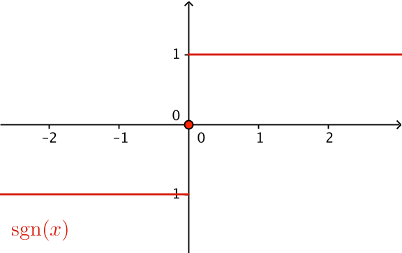
\includegraphics[scale =0.4]{im/SgnFktStetig.png}
    \end{minipage}
\end{example}

\begin{example}
    \begin{minipage}{0.6\textwidth}
        Die Betragsfunktion
        \begin{align*}
            |x| = \begin{cases}
                      x,  & \text{falls } x\geq 0 \\
                      -x, & \text{falls } x< 0    \\
                  \end{cases}
        \end{align*}
        ist stetig. Der Graph hat zwar einen „Spitz“, aber keine Sprungstelle.
        \begin{align*}
            \lim_{x\uparrow0}{\left|x\right|}=\lim_{x\downarrow0}{\left|x\right|}=\left|0\right|=0
        \end{align*}
    \end{minipage}
    \begin{minipage}{0.3 \textwidth}
        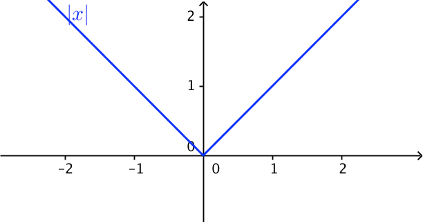
\includegraphics[scale =0.4]{im/BetragsFktStetig.png}
    \end{minipage}
\end{example}

\begin{example}
    \begin{minipage}{0.6\textwidth}
        Die Kehrwertfunktion  $p\left(x\right)=\frac{1}{x}$ ist trotz dem Sprung von $-\infty$ nach $+\infty$ stetig, weil die vermeintliche Sprungstelle $x=0$ ausserhalb des Definitionsbereichs $\mathbb{D}$ liegt.
    \end{minipage}
    \begin{minipage}{0.3 \textwidth}
        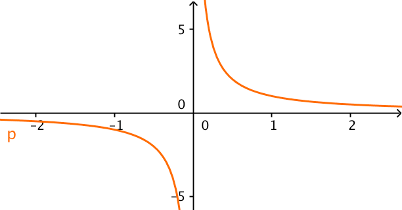
\includegraphics[scale =0.4]{im/1xStetig.png}
    \end{minipage}
\end{example}
\subsubsection{Übungen}
\begin{enumerate}
    \item Bestimmen Sie den links- und den rechtsseitigen Grenzwert der Funktion an der angegebenen Stelle. Ist die Funktion an dieser Stelle stetig?

          Bemerkung: Die Funktion $\lfloor x \rfloor$ ist die Abrundungsfunktion. Der Output ist die grösste ganze Zahl, die kleiner oder gleich $x$ ist.
          \begin{enumerate}
              \item $f(x)=x^2+x, \, a=3$
              \item  $f(x)=\lfloor x \rfloor, \, a=5$
              \item  $f(x)=\lfloor x-1 \rfloor, \, a=\frac{5}{2}$
              \item  $f(x)=\lvert x-5 \rvert, \, a=5$
              \item  $f(x)=\mathrm{sgn}(x-3), \, a=3$
              \item  $f(x)=\lfloor \cos(x)\rfloor, \, a=0$
          \end{enumerate}
    \item Gegeben ist die Funktion $f(x) = \left\{\begin{array}{ll}
                  3-x, & x<2 \\\frac{x}{2}+1, &x\ge 2
              \end{array}\right.$
          \begin{enumerate}
              \item Bestimme $\lim_{x\uparrow 4} f(x)$ und $\lim_{x\downarrow 4} f(x)$. Existiert $\lim_{x\to 4} f(x)$  ?
              \item Bestimme $\lim_{x\uparrow 2} f(x)$ und $\lim_{x\downarrow 2} f(x)$. Existiert $\lim_{x\to 2} f(x)$  ?
          \end{enumerate}
\end{enumerate}
\clearpage
\subsubsection*{Lösungen}
\begin{enumerate}
    \item Bestimme den links- und den rechtsseitigen Grenzwert der Funktion an der angegebenen Stelle. Ist die Funktion an dieser Stelle stetig?

          \begin{enumerate}
              \item $\lim\limits_{x \to 3^-} f(x) = 12$, \quad $\lim\limits_{x \to 3^+} f(x) = 12$ \newline $\Rightarrow$ Stetig
              \item $\lim\limits_{x \to 5^-} f(x) = 4$, \quad $\lim\limits_{x \to 5^+} f(x) = 5$ \newline $\Rightarrow$ Nicht stetig
              \item $\lim\limits_{x \to \frac{5}{2}^-} f(x) = 1$, \quad $\lim\limits_{x \to \frac{5}{2}^+} f(x) = 1$ \newline $\Rightarrow$  Stetig
              \item $\lim\limits_{x \to 5^-} f(x) = 0$, \quad $\lim\limits_{x \to 5^+} f(x) = 0$ \newline $\Rightarrow$ Stetig
              \item $\lim\limits_{x \to 3^-} f(x) = -1$, \quad $\lim\limits_{x \to 3^+} f(x) = 1$ \newline $\Rightarrow$ Nicht stetig
              \item $\lim\limits_{x \to 0^-} f(x) = 0$, \quad $\lim\limits_{x \to 0^+} f(x) = 0$ aber $\cos(0)=1$ \newline $\Rightarrow$ Nicht stetig
          \end{enumerate}

    \item Gegeben ist die Funktion
          \[
              f(x) = \begin{cases}
                  3-x,           & x<2     \\
                  \frac{x}{2}+1, & x\geq 2
              \end{cases}
          \]
          \begin{enumerate}
              \item $\lim\limits_{x \uparrow 4} f(x) = 3$, \quad $\lim\limits_{x \downarrow 4} f(x) = 3$ \newline $\Rightarrow$ Existiert mit Wert $3$
              \item $\lim\limits_{x \uparrow 2} f(x) = 1$, \quad $\lim\limits_{x \downarrow 2} f(x) = 2$ \newline $\Rightarrow$ Grenzwert existiert nicht
          \end{enumerate}
\end{enumerate}
\clearpage
\subsection{Asymptotische Analyse}
Bei einer `asymptotischen Analyse' werden die Grenzwerte einer Funktion für $x\to\pm\infty$ und an allen Definitionslücken bestimmt. Damit kann man sich eine gute Vorstellung des Funktionsgraphen machen.

\begin{example}
    {Asymptotische Analyse der Funktion $f(x)= \frac{x^2-4}{x^2-5x+6}$}{}
    \kariert{43}
\end{example}

\subsubsection{Übungen}
Führen Sie die asymptotische Analyse durch.
\begin{enumerate}
    \item $f(x) = \frac{x^2-2x-3}{x^2-9}$
    \item $g(x) = \frac{x}{x^3-4x^2+4x}$
\end{enumerate}

Zeichnen Sie die entsprechenden Graphen mit Geogebra, um die Lösung zu überprüfen.
\clearpage